\section{Aerosol Retrievals}

Aerosol Retrival Info Goes Here

From paper

The modeled radiances were computed with the SASKTRAN radiative transfer engine \citep{Bourassa2008a} for for High Resolution (SASKTRAN-HR) \citep{Zawada2015} measurements using the newly developed polarization module \citep{Dueck2015}. The model uses a given atmospheric state to solve the radiative transfer equation to determine the final radiance at the observer that follows
\begin{equation}
    I(s_{1}) = I(s_{0})e^{-\tau(s_{0}, s_{1})}+\int^{s_{1}}_{s_{0}}k(s)J(s)e^{-\tau(s, s_{1})}ds
\end{equation}
where $I(s_{1})$ is the radiance at the observer through a path from $s_{0}$ to $s_{1}$, the first term is the contribution of light that is attenuated along the line of sight from the sun to the observer at $s_{1}$. The second term takes the source term, $J(s)$, which is the radiance scattered into the line of sight and integrates the path along line of sight with attenuation to determine the scattering contribution to the final radiance. The extinction, given by $k(s)$, is the sum of the number density, $n(s)$, multiplied by the scattering cross section, $\sigma(s)$, over all species and $\tau$ is the optical depth. The polarized output of SASKTRAN-HR gives the Stokes vectors for the radiance on its internal coordinate grid which can be retrieved from the model and then rotated to match ALI's coordinate system.

The relative radiance level 1 data from ALI are used create a measurement vectors, $y$, in the following form
\begin{equation}
    \mathbf{y} = \log\left(\frac{\mathbf{I}(\mathbf{z},\lambda)}{I(z_{ref},\lambda)}\right)-\log\left(\frac{\mathbf{I}_{rayleigh}(\mathbf{z},\lambda)}{I_{rayleigh}(z_{ref},\lambda)}\right)
    \label{eqn:measurementVector}
\end{equation}
where $\mathbf{I}(\mathbf{z},\lambda)$ is the measured radiance from ALI and $I(z_{ref},\lambda)$ is the radiance at a reference altitude used to normalize the signal from a high altitude where there is little aerosol contribution, for ALI the highest possible altitude where the signal is above the noise threshold is around 25-30~km tangent height. The second term is modeled values from SASKTRAN-HR with only background neutral atmosphere to remove the rayleigh signal from the measured radiances which is done to improve the speed of the convergence of the retrieval. The ALI measurement vector is similar to the measurement vector used for the OSIRIS retrieval \citep{Bourassa2007,Bourassa2011}. A base aerosol state or a priori, $\mathbf{x}$, for aerosol extinction profile is used in the SASKTRAN-HR model. The forward model vector is constructed similarity to the measurement vector and follows.
\begin{equation}
    \mathbf{F}(\mathbf{x}) = \log\left(\frac{\mathbf{I}_{mod}(\mathbf{z},\lambda)}{I_{mod}(z_{ref},\lambda)}\right)-\log\left(\frac{\mathbf{I}_{rayleigh}(\mathbf{z},\lambda)}{I_{rayleigh}(z_{ref},\lambda)}\right)
    \label{eqn:forwardModel}
\end{equation}
where $I_{mod}(z,\lambda)$ is the modeled radiance for the measurement and $I_{mod}(z_{ref},\lambda)$ is the measurement at the same reference altitude for normalization. The forward model is used in combination with the measurement vector to update the extinction profile in the Multiplicative Algebraic Reconstruction Technique (MART) algorithm which was developed for use in the OSIRIS retrievals \citep{Bourassa2012a} with the following iterative technique
\begin{equation}
    x_{i+1} = x_{i}\sum_{j}\frac{y_{j}}{F(z_{j})}W_{ij}
\end{equation}
where $x_{i}$ is the aerosol extinction at each shell altitude, $i$ and $j$ is the tangent point from the measurements. $W_{ij}$ is the weighting matrix that relates the importance of each measurement vector to each shell altitude. This method was outlined by \cite{Degenstein2009} and allows for fast retrievals without calculating a Jacobian.

An error estimation was also needed to be able to fully classify the capabilities of ALI and was performed using a perturbation method. Once a retrieval has been completed for an image the result is used to estimate the error in the returned extinction. For each altitude, the measurement vector is perturbed by the error resulting form the level 0 to level 1 data conversion parameters used and from the readout electronics. The MART retrieval is rerun and the change of the extinction is determined. These are compiled to form a gain matrix, $\mathbf{G}$, with size is $n$ by $m$ which are the shell altitudes and the tangent altitudes grids respectively, with elements $g_{ij}$. The error at each retired altitude is then given by
\begin{equation}
    e_{i} = \left(\sum_{j}g_{ij}g_{ji}\right)^{0.5}
\end{equation}
which gives the error at at retrieved altitude.

Results:

In order to be able to use the ALI data in the MART method certain quantities were needed for the model; albedo, ozone concentration and cross sections, and aerosol cross sections. The albedo is required since an absolute radiance calibration was never preformed with ALI and the albedo cannot be determined directly form ALI's measurements, which is important since the amount of ground scatter in SASKTRAN-HR must correspond to the ground scatter during ALI's flight. Second, the ozone absorbtion features from the Chappuis band appear in the ALI measurements from 650 to 750~nm. The absorbtion must be accounted for to not artificially change the determined aerosol profiles. The ozone profiles were acquired from OSIRIS. Five scans that were within 48 hours of the balloon flight and  within 500~km of the launch facility were averaged together to be the ozone profile used in the SASKTRAN-HR model, with cross sections from \cite{Burrows1999}. The albedo is from the ADAM database which has monthly values for albedo over the surface on earth at a resolution of 0.1\si{\degree}~x~0.1\si{\degree} grid at 1~nm spectral resolution \citep{Muller2013}. The aerosol cross sections come from the Mie scattering derivation that was originally proposed by Mie and was implemented efficiently by \cite{Wiscombe1980}. For the purpose of the retrieval an a priori was used with a mode radius of 0.08~$\si{\micro\metre}$  and a mode width of 1.6 which is considered a standard size distribution for aerosol \citep{Deshler2003}.

The complete mission consisted of 216 images that were recorded in illuminated conditions. The MART retrieval method was run on a select signal set for the purpose of the analysis, specifically the last complete set of images from 650 to 950~nm consisting of images 204-216. They were chosen due to being the last in the mission and the sun was the highest in the sky giving the brightest atmosphere leading to the best signal to noise during the mission. A sample of the retrieval set can be observed in \autoref{fig:AliRetreivals} which highlights the 725, 825, and 925~nm retrievals. The left panels shows the measurement vector from ALI in black with the forward model radiance profile from SASKTRAN-HR in blue. For each of the wavelengths, the algorithm determines altitudes where the value of the measurement vector is less than the known noise and does not allow aerosol to be retrieved in those regions. Instead the scaling factor, given by $\alpha = yF^{-1}$ is scaled to the aerosol profile above and below the last retrieved point to keep the aerosol profile smooth, as discontinuities are nonphysical and can lead to a convergence failure in the MART algorithm. The middle panel shows the convergence between the measurement vector and the forward model result. For the center wavelengths, being 700-875~nm, a difference of less than 2\% is seen from 12 to 22~km with a few outliers.

The aerosol profile for the three wavelengths is shown in blue with the shading representing the error for the retrieval strictly based on measurement error and neglecting any model and atmospheric state errors. The green curve is the average 750~nm aerosol extinction profiles of the same five OSIRIS scans used for the ozone profile and red is the 750~nm aerosol extinction from SALOMON \citep{Berthet2002} which was launched from the Timmins balloon base as the Nimbus 5 mission on September 12, 2014. The aerosol extinction for ALI and OSIRIS are within 50\% of each other for a majority of the 725~nm and 825~nm profile while the upper altitude of the 925~nm are considerable different, in some places over 100\% difference occurs. However, agreement is best for 750~nm profile and displays a reasonable spectral dependance to also should be noted that the three instruments follow the same overall shape.  First, a bend in the profile occurs at approximately 25~km, then increases approximately linearly until 15~km where aerosol extinction leaves the linear trend and forms the peak of the measurement. The agreement in shape is an excellent result for the ALI mission due to the good numerical comparison with OSIRIS as well as the overall profile shape agreement between all three instruments.

\begin{figure}
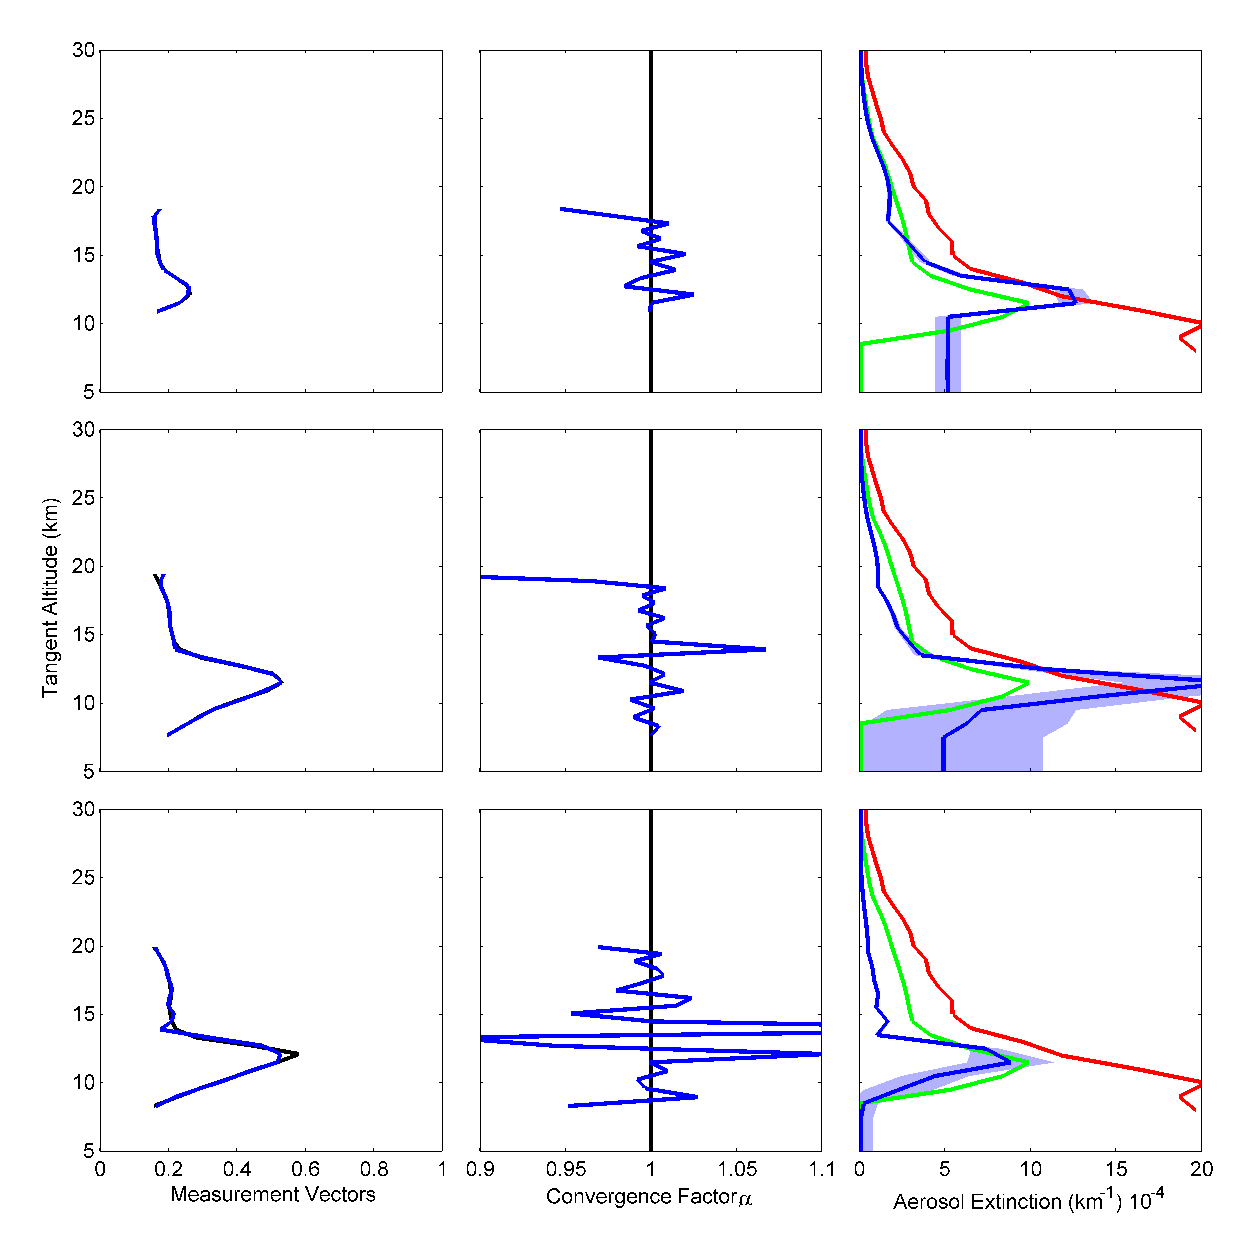
\includegraphics[width=1.0\textwidth]{./Images/5-3-AliRetreivals.pdf}
    \caption[TODO:Write This]{An example of three aerosol retrievals from images 207, 211, and 215, with center wavelengths of 725, 825, and 925~nm respectively and vertically displayed in the figure from top to bottom. The left column shows the measurement vector, $y$, in black with the retrieved forward model, $F$, in blue. The center column shows the ratio of the $y$ over $F$ known as $\alpha$ and is the convergence factor between the ALI measurement and the forward model. The final column is ALI aerosol extinction in blue with the associated error represented by the light blue shading. The green is 750~nm aerosol extinction measured by OSIRIS, and red is 750~nm extinction as measures by SALOMON.}
    \label{fig:5.3:AliRetreivals}
\end{figure} 